\documentclass[12pt]{article}
\usepackage[utf8]{inputenc}
\usepackage{float}
\usepackage{amsmath}


\usepackage[hmargin=3cm,vmargin=6.0cm]{geometry}
\topmargin=-2cm
\addtolength{\textheight}{6.5cm}
\addtolength{\textwidth}{2.0cm}
\setlength{\oddsidemargin}{0.0cm}
\setlength{\evensidemargin}{0.0cm}
\usepackage{indentfirst}
\usepackage{amsfonts}

\usepackage{graphicx}

\usepackage{listings}
\usepackage{xcolor}

\definecolor{codegreen}{rgb}{0,0.6,0}
\definecolor{codegray}{rgb}{0.5,0.5,0.5}
\definecolor{codepurple}{rgb}{0.58,0,0.82}
\definecolor{backcolour}{rgb}{0.95,0.95,0.92}

\lstdefinestyle{mystyle}{
  backgroundcolor=\color{backcolour},
  commentstyle=\color{codegreen},
  keywordstyle=\color{magenta},
  numberstyle=\tiny\color{codegray},
  stringstyle=\color{codepurple},
  basicstyle=\ttfamily\footnotesize,
  breakatwhitespace=false,
  breaklines=true,
  captionpos=b,
  keepspaces=true,
  numbers=none,
  numbersep=5pt,
  showspaces=false,
  showstringspaces=false,
  showtabs=false,
  tabsize=2
}

\lstset{style=myStyle}

\begin{document}

\section*{Student Information}

Name : Murat Bolu \\

ID : 2521300 \\


\section*{Answer 1}
\subsection*{a)}

Since the sample is small and the standard deviation of the population is
unknown, Student's \textit{t} distribution can be used. The critical value of
\textit{t} distribution is $\textit{t}_{\alpha/2} = \textit{t}_{0.01} = 2.602$
with $n-1=15$ degrees of freedom.

\begin{align*}
    \bar{X}&= \frac{8.4+7.8+6.4+6.7+6.6+6.6+7.2+4.1+
                    5.4+6.9+7.0+6.9+7.4+6.5+6.5+8.5}{16} \\[0.75ex]
    &= 6.806
\end{align*}

\begin{align*}
    s &= \sqrt{\frac{\sum_{i=1}^{n}(X_i - \bar{X})^2 }{n-1}} \\[0.75ex]
    &= \sqrt{\frac{\sum_{i=1}^{16}(X_i - 6.806)^2}{15}} \\[0.75ex]
    &= 1.055
\end{align*}

The 98\% confidence interval $\bar{X} \pm \textit{t}_{\alpha/2}
\frac{s}{\sqrt{n}}$ becomes $6.806 \pm 2.602 \cdot \frac{1.055}{4} =
[6.120,7.493]$.

\subsection*{b)}

Let $\mu_1$ be the initial gasoline consumption per 100 kilometers and $\mu_2$
be the improved gasoline consumption per 100 kilometers. Therefore, the null
hypothesis $H_0$ is $\mu_1 = \mu_2$ and the alternative hypothesis $H_A$ is
$\mu_1 > \mu_2$. Since we don't know the population standard deviation, we can
use T-statistic.

\begin{align*}
    \textit{t} &= \frac{\bar{X} - \mu}{s / \sqrt{n}} \\[0.75ex]
    &= \frac{6.806 - 7.5}{1.055 / 4} \\[0.75ex]
    &= -2.629
\end{align*}

The rejection region is $R = (-\infty, -\textit{t}_{\alpha}] = (-\infty,
-\textit{t}_{0.05}] = (-\infty, -1.753]$ with 15 degrees of freedom, since we
are using a left-tail alternative. Since $t \in R$, we can reject the null
hypothesis. There is sufficient evidence that the improvement was effective.

\subsection*{c)}

Since $\bar{X} = 6.806 > 6.5$, we can immediately accept the null hypothesis
because the T-statistic is positive and the rejection region includes zero.

\section*{Answer 2}
\subsection*{a)}

The null hypothesis $H_0$ should be considered to be that the rent prices stayed
the same. The alternative hypothesis $H_A$ then becomes the rent prices have
increased.

\subsection*{b)}

Since the population standard deviation is known, Z-statistic can be used.

\begin{align*}
    Z &= \frac{\bar{X}-\mu}{\sigma / \sqrt{n}} \\[0.75ex]
    &= \frac{5500 - 5000}{2000 / 10} \\[0.75ex]
    &= \frac{500}{200} \\[0.75ex]
    &= 2.5
\end{align*}

The rejection region is $R = [\textit{z}_{\alpha}, \infty) = [\textit{z}_{0.05},
\infty) = [1.645, \infty)$, since we are using a right-tail alternative. Since
$Z \in R$, we can reject the null hypothesis. There is sufficient evidence that
the rent prices have increased. Ahmet can claim that there is an increase in the
rent prices compared to the last year at 5\% level of significance.

\subsection*{c)}

The \textit{P}-value is $\textit{P} = \textbf{\textit{P}}\{Z \geq Z_\text{obs}\}
= \textbf{\textit{P}}\{Z \geq 2.5\} = 1 - \Phi(2.5) = 0.0062$. This means Ahmet
can claim that the rent prices have increased with 0.62\% level of significance.

\subsection*{d)}

The null hypothesis $H_0: \mu_A = \mu_I$ is that the rent prices in Ankara,
$\mu_A$, are the same as the rent prices in Istanbul, $\mu_I$. The alternative
hypothesis $H_A: \mu_A < \mu_I$ is that the rent prices in Ankara are lower than
the rent prices in Istanbul. Since we know both of the standard deviations, we
can use Z-statistic.

\begin{align*}
    Z &= \frac{\bar{X} - \bar{Y} - D}
              {\sqrt{\frac{\sigma_X^2}{n}+\frac{\sigma_Y^2}{m}}} \\[0.75ex]
    &= \frac{5500 - 6500 - 0}
            {\sqrt{\frac{2000^2}{100}+\frac{3000^2}{60}}} \\[0.75ex]
    &= \frac{-1000}{\sqrt{40,000+150,000}} \\[0.75ex]
    &= -\frac{1000}{435.890} \\[0.75ex]
    &= -2.294
\end{align*}

We can calculate the \textit{P}-value as $\Phi(-2.294) = 0.011$. Since the
\textit{P}-value is barely above 1\%, the null hypothesis should be accepted.
Therefore, they cannot claim that the prices in Ankara are lower than the prices
in Istanbul.


\section*{Answer 3}

Let's construct the table and calculate the sums for all rows and columns.

\begin{center}
\begin{tabular}{c|c c c c|c}
Obs$(i,j)$    & Winter & Spring & Summer & Autumn & $n_{i \cdot}$ \\
\hline
Rainy         & 34 & 32 & 15 & 19 & 100 \\
Non-rainy     & 56 & 58 & 75 & 71 & 260 \\
\hline
$n_{\cdot j}$ & 90 & 90 & 90 & 90 & 360 \\
\end{tabular}
\end{center}

Now, we can construct the table for expected number days being rainy and
non-rainy if they were independent of season.

\begin{center}
\begin{tabular}{c|c c c c|c}
$\widehat{\text{Exp}}(i,j)$
              & Winter & Spring & Summer & Autumn & $n_{i \cdot}$ \\
\hline
Rainy         & 25 & 25 & 25 & 25 & 100 \\
Non-rainy     & 65 & 65 & 65 & 65 & 260 \\
\hline
$n_{\cdot j}$ & 90 & 90 & 90 & 90 & 360 \\
\end{tabular}
\end{center}

Now, we can calculate Chi-square statistic.

\begin{align*}
    \chi^2_\text{obs} =\ &\frac{(34-25)^2}{25} + \frac{(32-25)^2}{25}
                      +   \frac{(15-25)^2}{25} + \frac{(19-25)^2}{25} \\[0.75ex]
                      +\ &\frac{(56-65)^2}{65} + \frac{(58-65)^2}{65}
                      +   \frac{(75-65)^2}{65} + \frac{(71-65)^2}{65} \\[0.75ex]
    =\ &\frac{81+49+100+36}{25} + \frac{81+49+100+36}{65} \\[0.75ex]
    =\ &\frac{266}{25} + \frac{266}{65} \\[0.75ex]
    =\ &\frac{3458+1330}{325} \\[0.75ex]
    =\ &14.732
\end{align*}

We have $(4-1)\cdot(2-1) = 3$ degrees of freedom. Accounting into three degrees
of freedom, we can find the \textit{P}-value by $\textit{P} =
\textbf{\textit{P}}\{\chi^2 \geq 14.732\} < 0.005$. We have a significant
evidence that the number of rainy days depends on the season, with a
significance level above 99.5\%, because \textit{P}-value is less than $0.005$.

\section*{Answer 4}

\noindent
The Octave code is as follows,
\begin{lstlisting}[language=Octave]
% Load statistics module for chi-square independence test
pkg load statistics;

% Define the matrix
X = [34 32 15 19; 56 58 75 71];

% Use library function
[pval, chisq, df] = chisquare_test_independence(X)
\end{lstlisting}

\noindent
with a screenshot of some outputs,

\begin{center}
  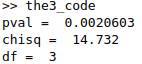
\includegraphics[scale = 1]{the3_output.png}
\end{center}

The findings agree with our calculations.

\end{document}
